\documentclass[a4paper, fleqn]{article}
\usepackage{header}

\usetikzlibrary{patterns}
\usepgfplotslibrary{fillbetween}
\pgfplotsset{compat=1.17}

\title{Семинарский лист 2.3}
\author{
    % Александр Богданов   \\ \href{https://t.me/SphericalPotatoInVacuum}{Telegram} \and
    % Алиса Вернигор       \\ \href{https://t.me/allisyonok}{Telegram} \and
    Анастасия Григорьева \\ \href{https://t.me/weifoll}{Telegram} \and
    % Василий Шныпко       \\ \href{https://t.me/yourvash}{Telegram} \and
    % Данил Казанцев       \\ \href{https://t.me/vserosbuybuy}{Telegram} \and
    Денис Козлов         \\ \href{https://t.me/DKozl50}{Telegram} \and
    Елизавета Орешонок   \\ \href{https://t.me/eaoresh}{Telegram} \and
    Ира Голобородько     \\ \href{https://t.me/Ira4kgl}{Telegram}
    % Иван Пешехонов       \\ \href{https://t.me/JohanDDC}{Telegram} \and
    % Иван Добросовестнов  \\ \href{https://t.me/ivankot13}{Telegram} \and
    % Настя Городилова     \\ \href{https://t.me/nastygorodi}{Telegram} \and
    % Никита Насонков      \\ \href{https://t.me/nnv_nick}{Telegram} \and
    % Сергей Лоптев        \\ \href{https://t.me/beast_sl}{Telegram}
}

\date{Версия от {\ddmmyyyydate\today} \currenttime}

\begin{document}
    \maketitle
    
    \section*{Предполагая функцию $f$ непрерывной на $D$, приведите двойной интеграл от $f$ по $D$ к повторному 
    двумя способами: по $x$ затем по $y$ и наоборот.}
    \subsection*{Задача 1\\[-40 pt]}
    \begin{align*}
        & D = \{ (x, y) \,|\, x, y \in [0; 1], x^2 + y^2 \ge 1 \} \\[3 pt]
        & \text{Множество точек, находящихся в квадрате, ограниченном прямыми $x = 0, x = 1, y = 0, y = 1$,} \\
        & \text{за пределами круга радиуса 1 с центром в точке $(0, 0)$:} \\[3 pt]
    \end{align*}
        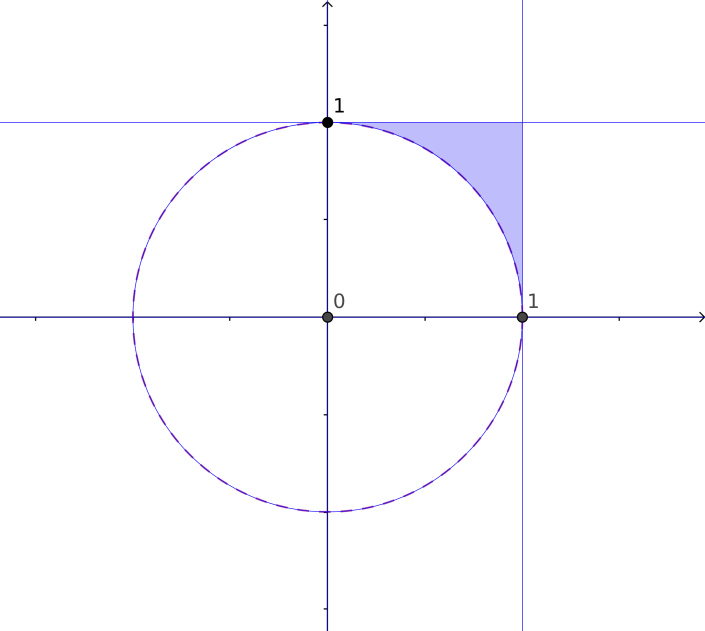
\includegraphics[width=8cm, height=7cm]{list23imgs/task 1.png}\\
    \begin{align*}
        & \text{Интеграл по $x$ затем по $y$:} \\
        & \int\limits_0^1 dy \!\!\! \int\limits_{\sqrt{1-y^2}}^1 \!\!\! dx = \int\limits_0^1 dy \cdot x \Bigm|_{\sqrt{1-y^2}}^1
        = \int\limits_0^1 dy \left( 1 - \sqrt{1-y^2} \right) = \int\limits_0^1 dy - \int\limits_0^1 \sqrt{1-y^2} \, dy 
        = 1 - \int\limits_0^1 \sqrt{1-y^2} \, dy \\
        & \text{Замена: } y = \sin u \Leftrightarrow \int\limits_0^1 \sqrt{1-y^2} \, dy 
        = \int\limits_0^{\frac{\pi}2} \cos u \, \sqrt{1-\sin^2 u} \, du = \int\limits_0^{\frac{\pi}2} \cos^2 u \, du 
        = \int\limits_0^{\frac{\pi}2} \frac{\cos 2u + 1}2 \, du = \\
        & = \frac12 \int\limits_0^{\frac{\pi}2} \cos 2u \, du + \frac12 \int\limits_0^{\frac{\pi}2} \! du 
        = \frac14 \, \sin 2u \Bigm|_0^{\frac{\pi}2} + \frac12\, u \Bigm|_0^{\frac{\pi}2} = \frac{\pi}4 \\
        & \text{Тогда:} \\
        & \int\limits_0^1 dy \!\!\! \int\limits_{\sqrt{1-y^2}}^1 \!\!\! dx = 1 - \frac{\pi}4 \\
        & \text{Очевидно, что повторный интеграл, взятый в другом порядке, будет вычисляться точно так же:} \\
        & \int\limits_0^1 dx \!\!\! \int\limits_{\sqrt{1-x^2}}^1 \!\!\! dy = \int\limits_0^1 dy \cdot y \Bigm|_{\sqrt{1-x^2}}^1
        = \int\limits_0^1 dx \left( 1 - \sqrt{1-x^2} \right) = \int\limits_0^1 dy - \int\limits_0^1 \sqrt{1-x^2} \, dy 
        = 1 - \frac{\pi}4 \\
        & \text{\fbox{Ответ: $1 - \dfrac{\pi}4$.}}
    \end{align*}
    
    \subsection*{Задача 2}
    \begin{align*}
        & D = \{ (x, y) \,|\, x, y \in [0; 1], (x - 1)^2 + (y - 1)^2 \ge 1 \} \\[3 pt]
        & \text{Множество точек, находящихся в квадрате, ограниченном прямыми $x = 0, x = 1, y = 0, y = 1$,} \\
        & \text{за пределами круга радиуса 1 с центром в точке $(1, 1)$:} 
        \end{align*}
        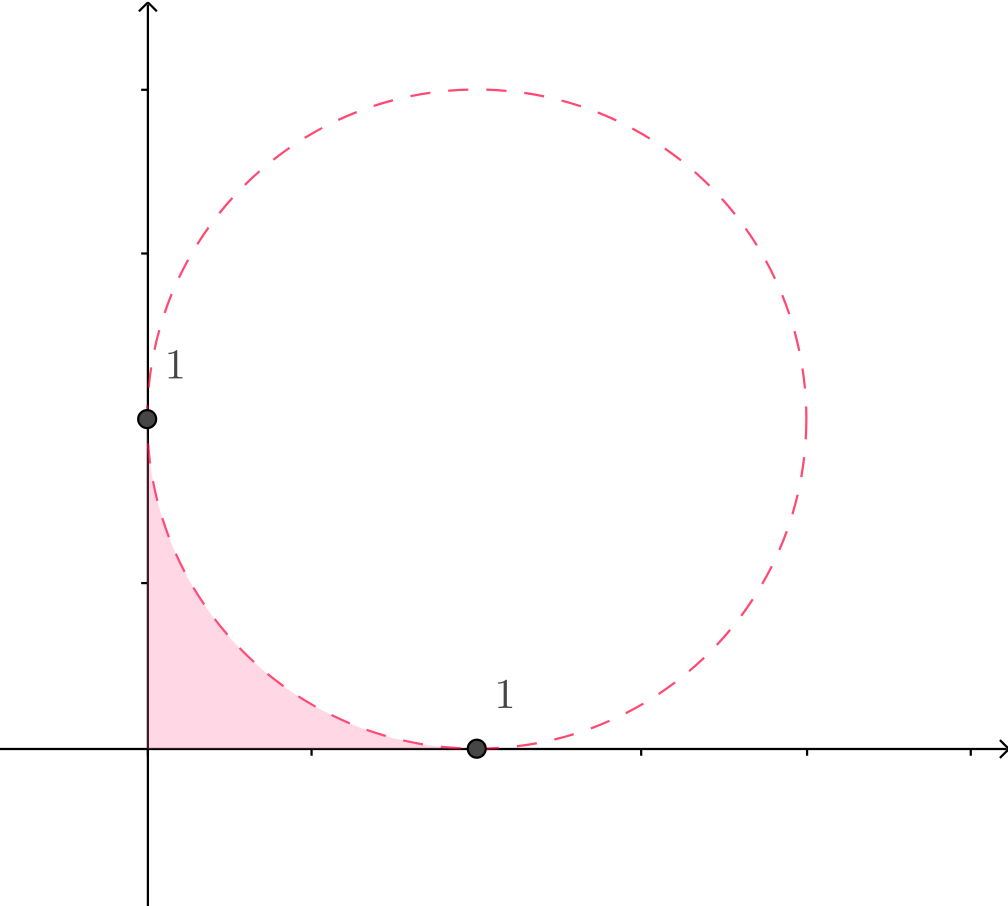
\includegraphics[width=8cm, height=7cm]{list23imgs/task 2.png}\\
        \begin{align*}
        & \text{Интеграл по $x$ затем по $y$:} \\
        & \int\limits_0^1 dy \!\!\! \int\limits_0^{\sqrt{1-(y-1)^2}+1} \!\!\! dx 
        = \int\limits_0^1 dy \cdot x \Bigm|_0^{\sqrt{1-(y-1)^2}+1} = \int\limits_0^1 dy \left( \sqrt{1-(y-1)^2} + 1 \right) 
        = \int\limits_0^1 \sqrt{1-(y-1)^2} \, dy + 1 \\
        & \text{Замена: } (y-1) = \sin u \Leftrightarrow \int\limits_0^1 \sqrt{1-(y-1)^2} \, dy 
        = \int\limits_0^{\frac{\pi}2} \cos u \, \sqrt{1-\sin^2 u} \, du = \int\limits_{-\frac{\pi}2}^0 \cos^2 u \, du 
        = \int\limits_{-\frac{\pi}2}^0 \frac{\cos 2u + 1}2 \, du = \\
        & = \frac12 \int\limits_{-\frac{\pi}2}^0 \cos 2u \, du + \frac12 \int\limits_{-\frac{\pi}2}^0 \! du 
        = \frac14 \, \sin 2u \Bigm|_{-\frac{\pi}2}^0 + \frac12\, u \Bigm|_{-\frac{\pi}2}^0 = -\frac{\pi}4 \\
        & \text{Тогда:} \\
        & \int\limits_0^1 dy \!\!\! \int\limits_0^{\sqrt{1-(y-1)^2}+1} \!\!\! dx = 1 - \frac{\pi}4 \\
        & \text{Очевидно, что повторный интеграл, взятый в другом порядке, будет вычисляться точно так же:} \\
        & \int\limits_0^1 dx \!\!\! \int\limits_0^{\sqrt{1-(x-1)^2}+1} \!\!\! dy = \int\limits_0^1 \sqrt{1-(x-1)^2} \, dx + 1
        = 1 - \frac{\pi}4 \\
        & \text{\fbox{Ответ: $1 - \dfrac{\pi}4$.}}
    \end{align*}
    
    \subsection*{Задача 3}
    
    $D = \{ (x,y ) \mid x^2 + 2 y^2 \leq 16, \; x^2 - y^2 \leq 1\}.$
    
    
    $\bullet$ $ x^2 + 2 y^2 = 16$ -- эллипс, нужны точки внутри него;
    
    $\bullet$ $x^2 - y^2 = 1$ -- гипербола, нужна область, ограниченная двумя частями ее графика. 
    
    
    Найдем координаты точки пересечения кривых: $\begin{cases} x ^ 2 + 2 y^2 = 16;
    x^2  - y^2 = 1;\end{cases} \implies \begin{cases} y = \pm \sqrt{5}; \\ x = \pm \sqrt{6} .\end{cases}$
    
    Эллипс пересекает ось ординат в точках $(0, \sqrt{8})$ и $(0, -\sqrt{8}).$ 
    
    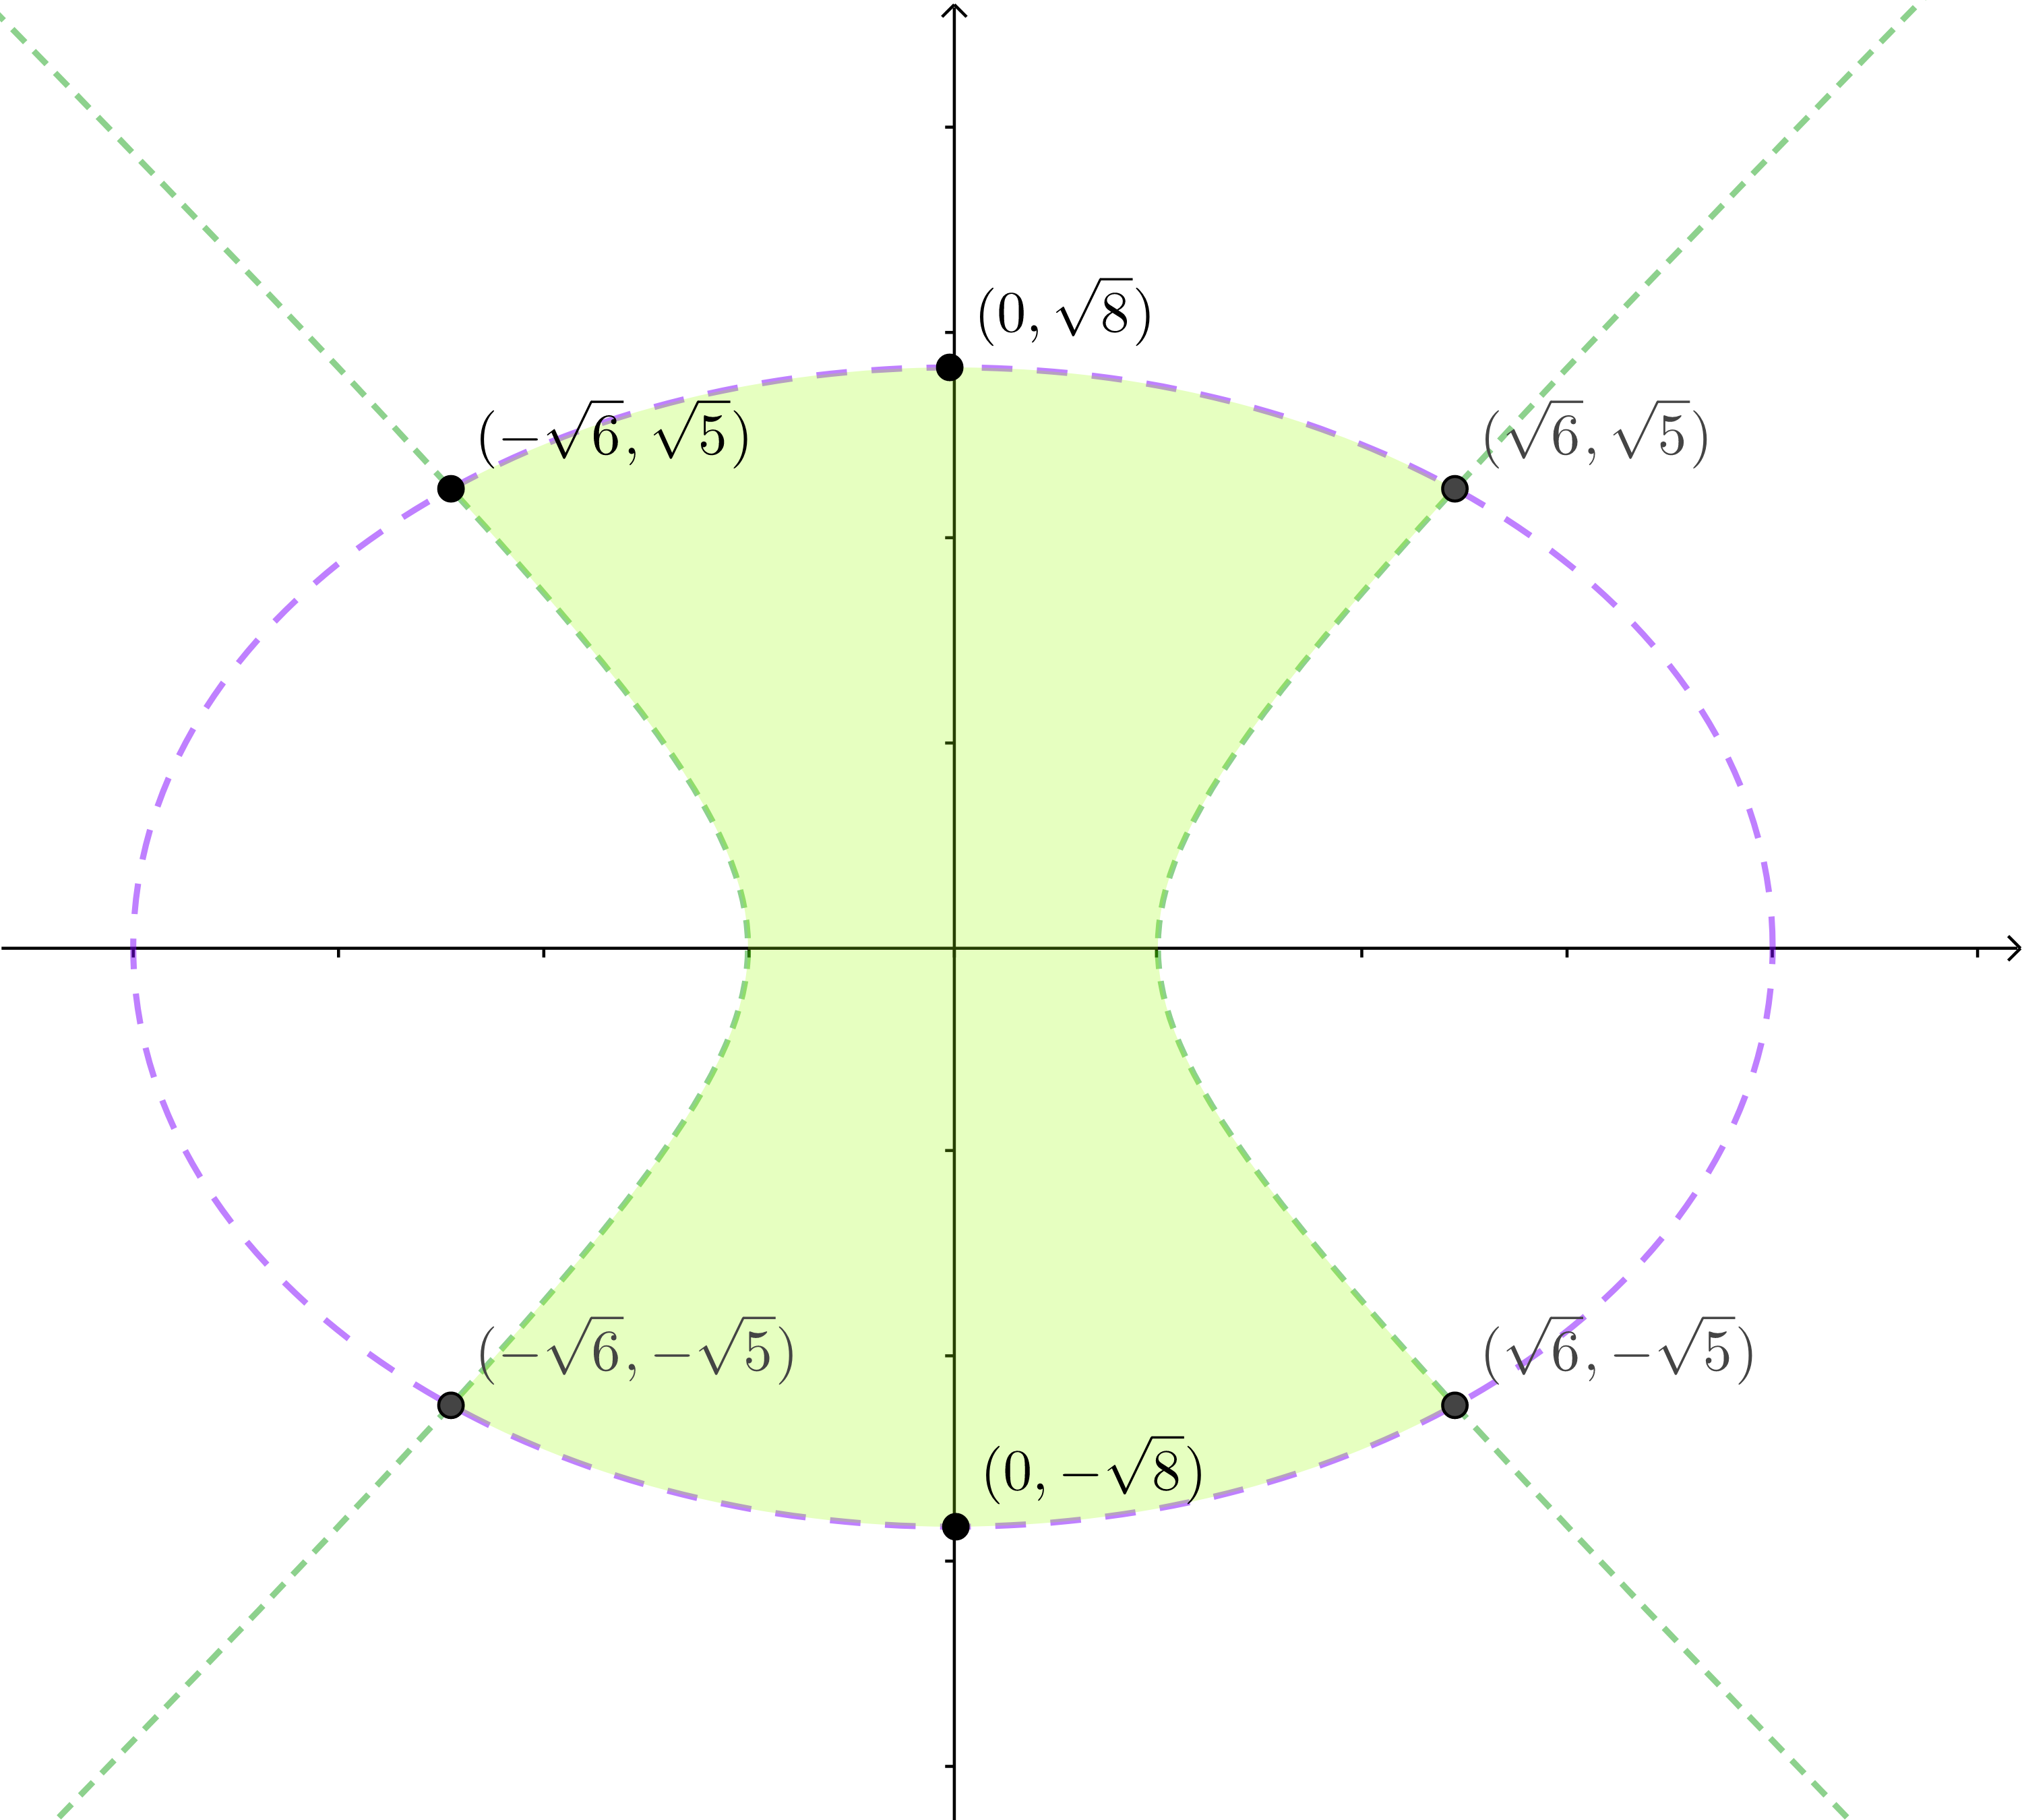
\includegraphics[width=11cm, height=10cm]{list23imgs/task 3.png}
    
    
    Интегрируя по $x$, видим два симметричных относительно 0 куска $\implies$ можем рассмотреть любой из них и продублировать интеграл.
    
    Интегрируем правую часть -- интеграл разбивается на участки до перекрытия гиперболой (до координаты 1) и после. Во втором интеграле используем симметричность относительно $Ox.$
    
    
    
    Итого: $I(D, f) = 2 \cdot \left( \displaystyle \int\limits_0^{1} dx \int\limits_{-\sqrt{(16 - x^2)/2}}^{\sqrt{(16 - x^2)/2} } f(x,y) dy + 2 \cdot \displaystyle \int\limits_1^{\sqrt{6}} dx \int\limits_{\sqrt{x^2 - 1}}^{\sqrt{(16 - x^2)/2} } f(x, y) dy \right).$
    
    Теперь по $y$. Тоже используем симметричность и считаем лишь верхнюю часть.
    
     $I(D,f ) = 2 \cdot \left( \displaystyle \int\limits_0^{\sqrt{5}} dy \int\limits_{-\sqrt{1 + y^2}}^{\sqrt{1 + y^2} } f(x, y) dx + \displaystyle \int\limits_{\sqrt{5}}^{\sqrt{8}} dy \int\limits_{-\sqrt{16 - 2y^2}}^{\sqrt{16 - 2y^2} } f(x, y) dx \right).$
    
     \subsection*{Задача 4}
        
    $D = \{ (x,y ) \mid x, y \geq 0, \; 0< xy \leq 1, \; y \leq 2x, \; x \leq 2y\}.$
    
    $\bullet$ $xy = 1$ -- гипербола, рассматривается участок под ней;
    
    $\bullet$ $y = 2x$ -- прямая, рассматривается полуплоскость под ней;
    
    $\bullet$ $x = 2y$ -- прямая, рассматривается полуплоскость над ней.
    
    Найдем точки пересечения кривых: $\begin{cases} xy = 1;\\
    y = 2x; \end{cases} \implies\begin{cases} y = \sqrt{2}; \\  x = \sqrt{2}/2 ;\end{cases}\; \; \begin{cases}xy = 1;\\
    x = 2y;\end{cases}\implies\begin{cases}y = \sqrt{2}/2; \\  x = \sqrt{2} .\end{cases}$
    
    Значит, требуется привести интеграл по следующему множеству:
    
    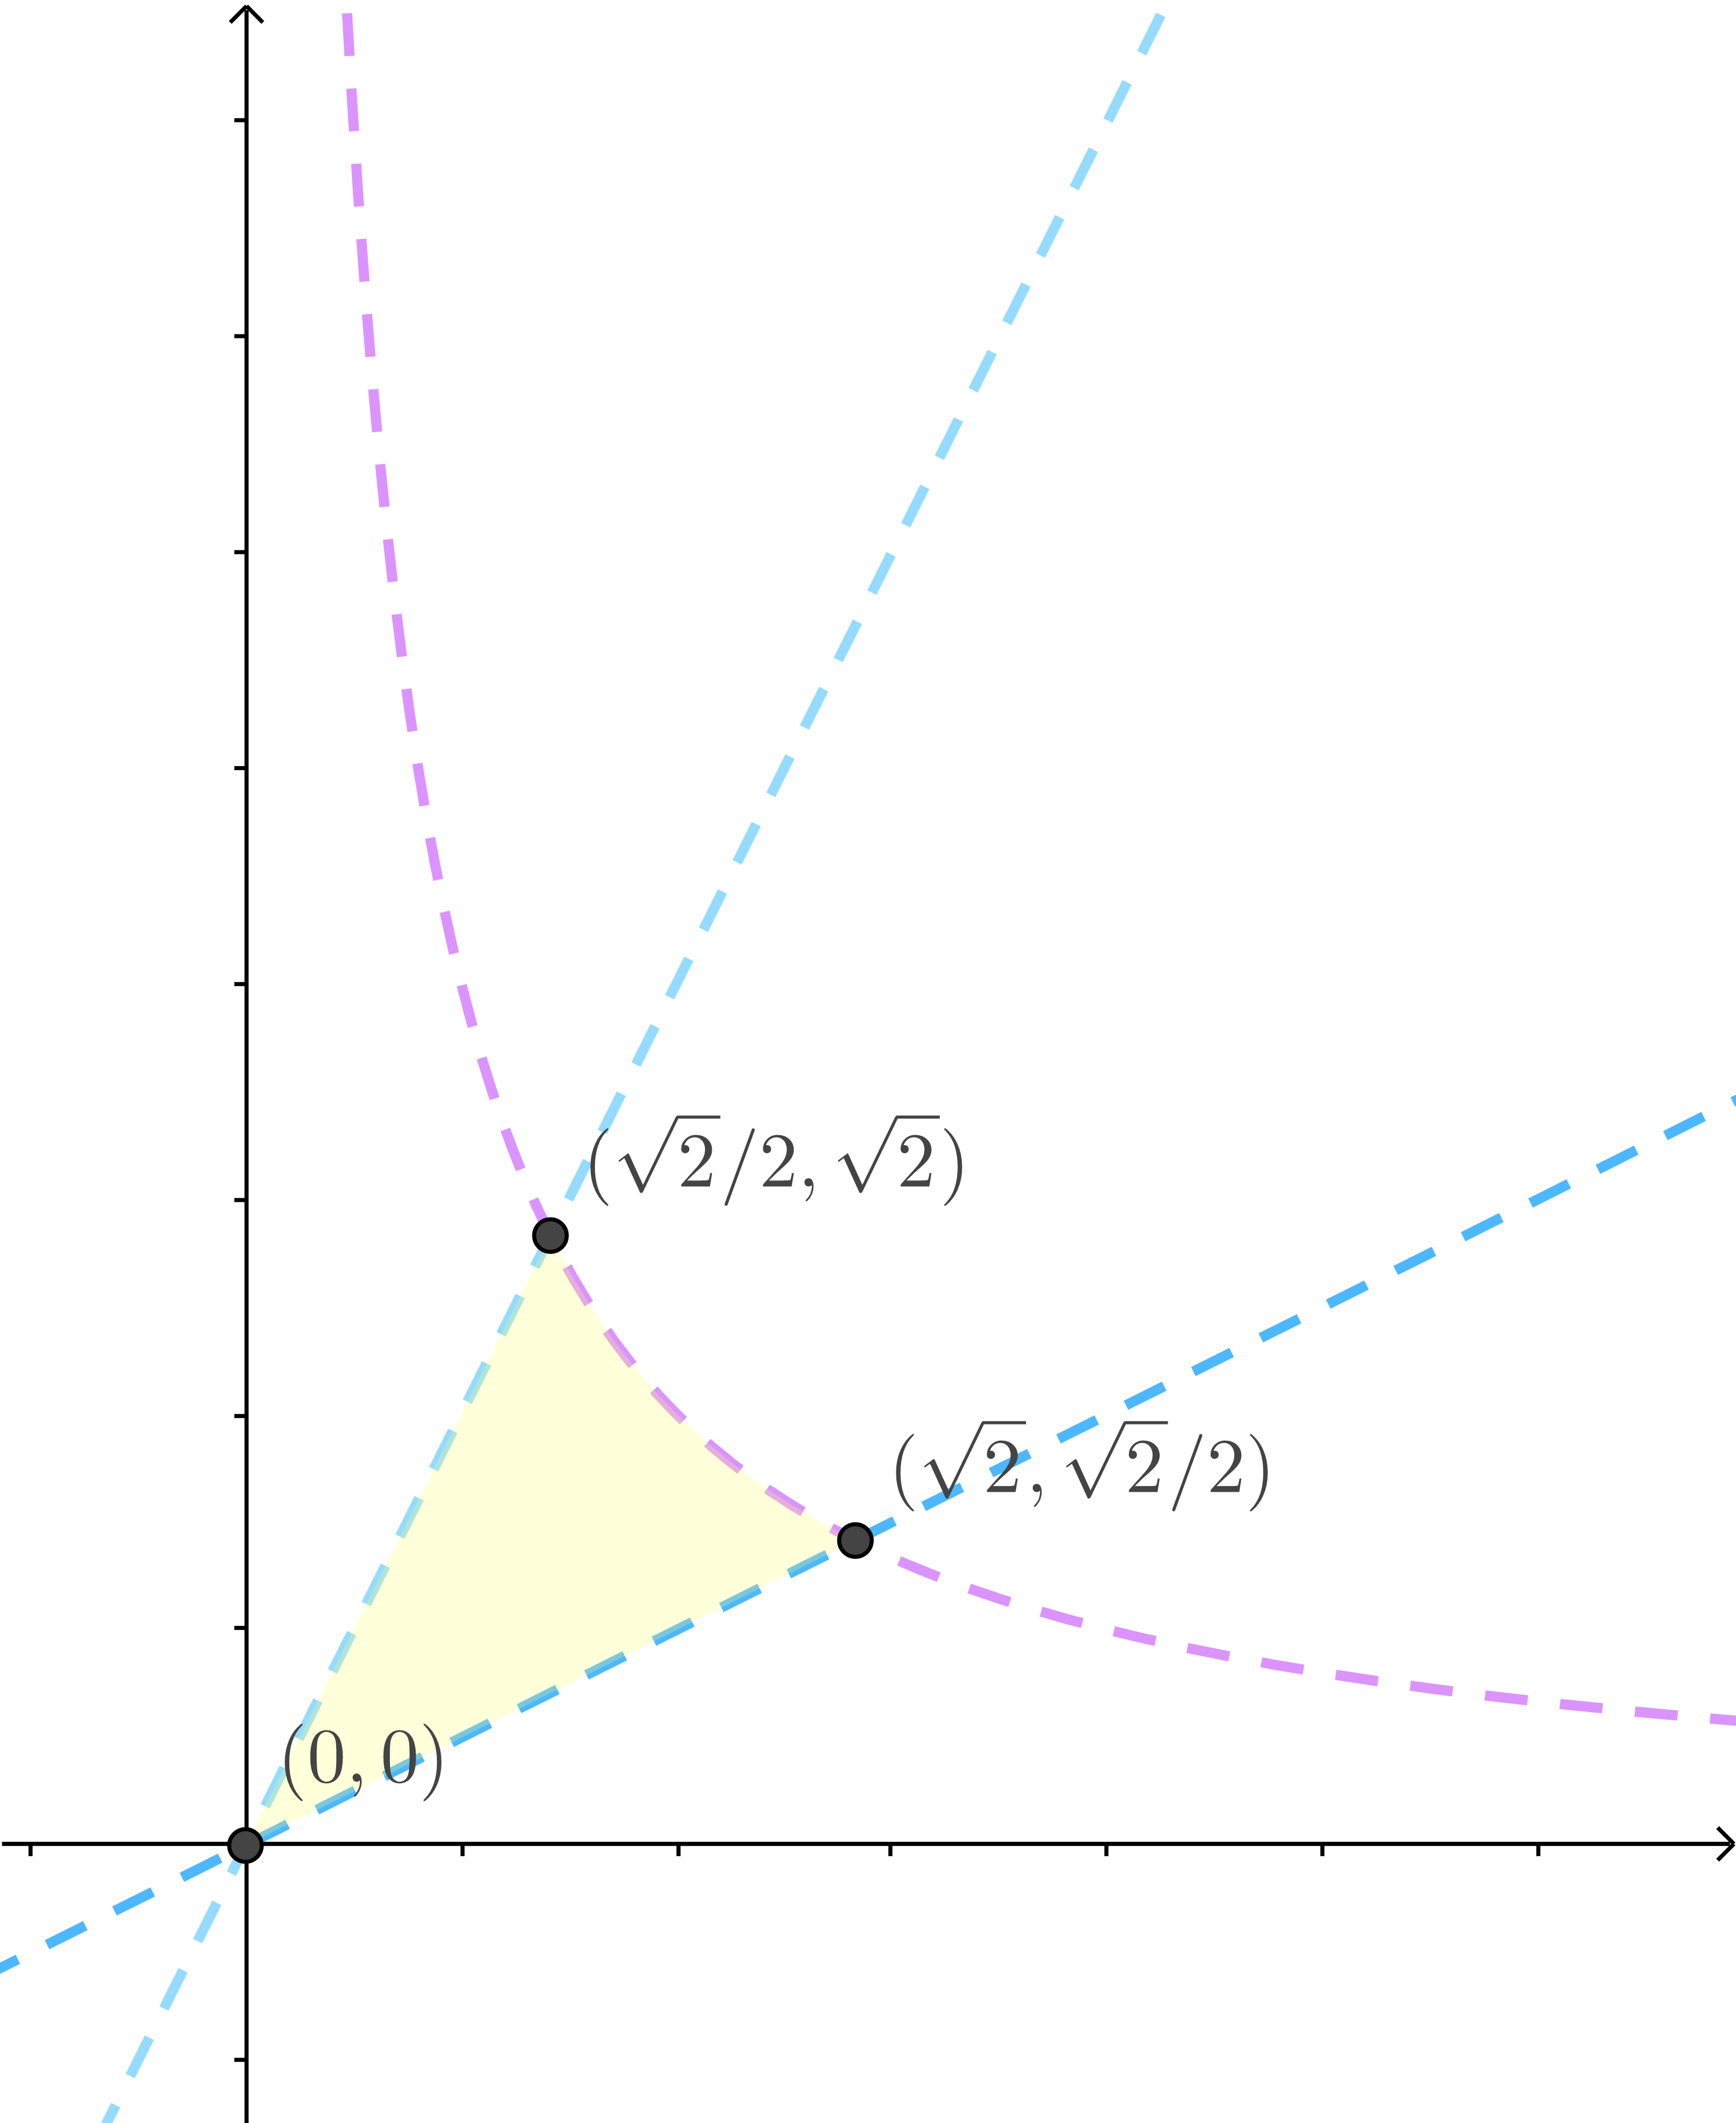
\includegraphics[width=8cm, height=9cm]{list23imgs/task 4.png}
    
    Разбивая область интегрирования по $x$ до перекрытия с гиперболой и после, получаем:
    
    $I(D, f) = \displaystyle \int\limits_{0}^{\sqrt{2}/2}dx \int\limits_{x/2}^{2x} f(x, y)dy + \displaystyle \int\limits_{\sqrt{2}/2}^{\sqrt{2}}dx \int\limits_{x/2}^{1/x} f(x, y)dy$;
    
    Разбивая область интегрирования по $y$ до перекрытия с гиперболой и после, получаем (симметрично):
    
    $I(D, f) = \displaystyle \int\limits_{0}^{\sqrt{2}/2}dy \int\limits_{x/2}^{2x} f(x, y)dx + \displaystyle \int\limits_{\sqrt{2}/2}^{\sqrt{2}}dy \int\limits_{x/2}^{1/x} f(x, y)dx$.
    
    \section*{Предполагая функцию $f$ непрерывной на $D$, измените порядок интегрирования в повторном интеграле}
    \subsection*{Задача 5}
    
    $\int\limits_{0}^{1} dy \int\limits_{0}^{2y - y^2} f(x,y)dx.$
    
    Чтобы изменить порядок интегрирования, нужно восстановить множество $D$. Это можно сделать, изучив пределы интегрирования.
    
    $y \in [0, 1]$ -- судя по внешнему интегралу.
    
    Нас интересуют точки с положительной абсциссой, которые лежат слева от кривой $x = 2y - y^2.$ Парабола пересекается с $Oy$ в $(0, 0)$ и $(0,2)$, и имеет вершину  в $(1,1).$
    
    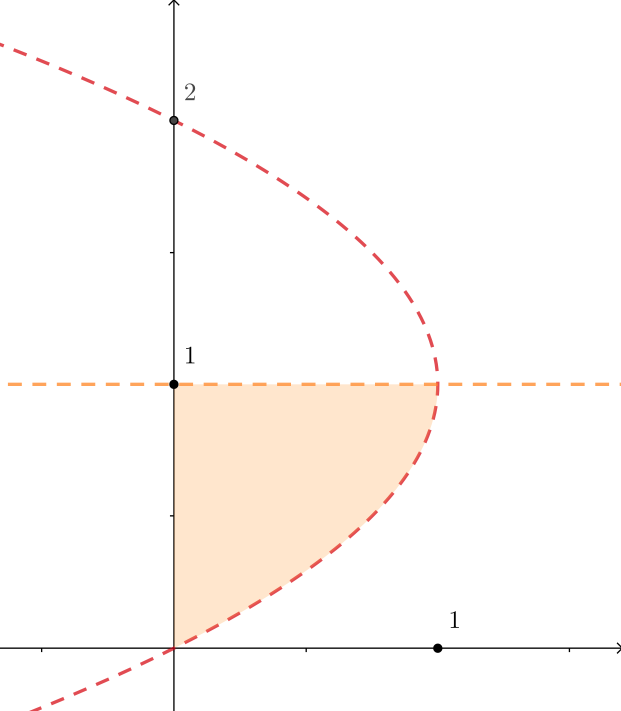
\includegraphics[width=8cm, height=9cm]{list23imgs/task_5.png}

    
    $x = 2y - y^2 \iff y = 1 \pm \sqrt{1 - x}.$ Но наш кейс -- только $y = 1 - \sqrt{1 - x},$ так как $y \in [0,1].$
    
    $x \in [0,1]$  -- нам это нужно для пределов внешнего интеграла.
    
    Далее задача сводится к тому, что мы уже умеем.
    
    Итого: $\int\limits_{0}^{1}dx \int\limits_{1 - \sqrt{1 - x}}^{1} f(x, y)dy.$

    \subsection*{Задача 6}
    \begin{flalign*}
        & \int_0^1 dy \int_{\frac{y^2}{9}}^{y} f(x, y) dx + 
        \int_1^3 dy \int_{\frac{y^2}{9}}^1 f(x, y) dx = \text{ пристально смотрим на рисунок } = \\
        & = \int_0^1 \int_{x}^{3\sqrt{x}} f(x, y) dx dy = 
        \int_0^1 dx \int_{x}^{3\sqrt{x}} f(x, y) dy 
    \end{flalign*}
    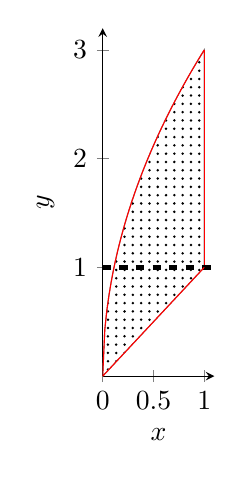
\begin{tikzpicture} 
        \begin{axis}[axis lines=center, xlabel={$x$}, ylabel={$y$}, % служебные строки
                        xlabel near ticks, ylabel near ticks, hide obscured x ticks=false, % служебные строки
                        xmin=0, xmax=1.1, ymin=0, ymax=3.2, % диапазон значений
                        width=3cm, height=6cm] % размер картинки
            % чтобы рисовать линии по координатам (x, y) используйте (axis cs:x, y), как здесь:
            \draw[color=red] (axis cs:1, 1) -- (axis cs:1, 3); % вертикальная линия справа
            \draw[dashed, line width=2pt, color=black] (axis cs:0, 1) -- (axis cs:1.1, 1); % деление двух интегралов
            % чтобы заполнить площадь между графиками стоит дать графикам имена (здесь A и B):
            \addplot [name path=A, domain=0:1, color=red] {x}; 
            \addplot [name path=B, domain=0:1, color=red, samples=50] {sqrt(x)*3}; % тикз умеет в математику
            \addplot [pattern=dots, draw=gray] fill between[of=A and B]; % само заполнение через fill between
        \end{axis} 
    \end{tikzpicture} 

    \subsection*{Задача 7}
    
    $\int\limits_{3}^{7} dy \int\limits_{9/y}^{3}f(x,y)dx +\int\limits_{7}^{9} dy \int\limits_{9/y}^{10 - y}f(x,y)dx. $
    
    $y \in [3, 9].$
    
    При $y \in [3,7]$ точки лежат между графиком гиперболы $y = 9/x$ и прямой $x = 3$.
    
    При $y \in [7,9]$ точки лежат между графиком гиперболы $y = 9/x$ и прямой $y = -x + 10$.
    
    Найдём точки пересечения кривых:
    
    $\begin{cases}
    x = 3;\\
    y = -x + 10
    \end{cases} \implies
    \begin{cases}
    x = 3;\\
    y = 7
    \end{cases}$ $\begin{cases}
    y = 9/x;\\
    y = -x + 10
    \end{cases} \implies
    \begin{cases}
    x = 1;\\
    y = 9
    \end{cases}$ $\begin{cases}
    y = 9/x;\\
    x = 3
    \end{cases} \implies
    \begin{cases}
    x = 3;\\
    y = 3
    \end{cases}$ 
    
    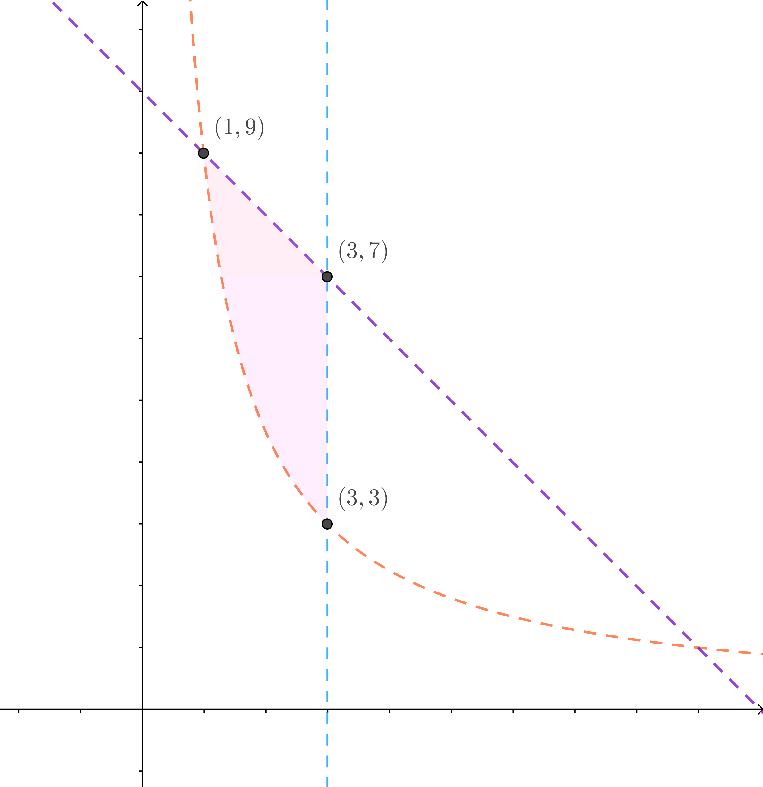
\includegraphics[width=8cm, height=9cm]{list23imgs/task 7.png}
    
    Теперь изменим порядок интегрирования. $x \in [1, 3].$ При всех $x$ точки лежат между гиперболой и прямой $y = -x + 10.$
    
    Итого: $I(D, f) = \int\limits_{1}^{3} dx \int\limits_{9/y}^{10 - y} f(x, y) dy$
    
    \subsection*{Задача 8}
    
    $\displaystyle\int\limits_{0}^{1} dy \int\limits_{\sqrt{4 - 4 y}}^{\sqrt{4 - y^2}} f(x, y) dx + 
    \int\limits_{1}^{2} dy \int\limits_{0}^{\sqrt{4 - y^2}} f(x, y) dx.$

    Восстанавливаем  $D$. 
    
    $y \in [0, 2].$ На промежутке $y \in [0,1]$ нас интересуют точки между параболой $y = 1 - x^2/4$ и окружностью $x^2 + y^2 = 4.$ На промежутке $y \in [1,2]$ нас интересуют точки между началом координат и окружностью $x^2 + y^2 = 4$.
    
    Радиус окружности 2, вершина параболы $(0, 1),$ пересечение с $Ox$ в точке $(2, 0).$
    
    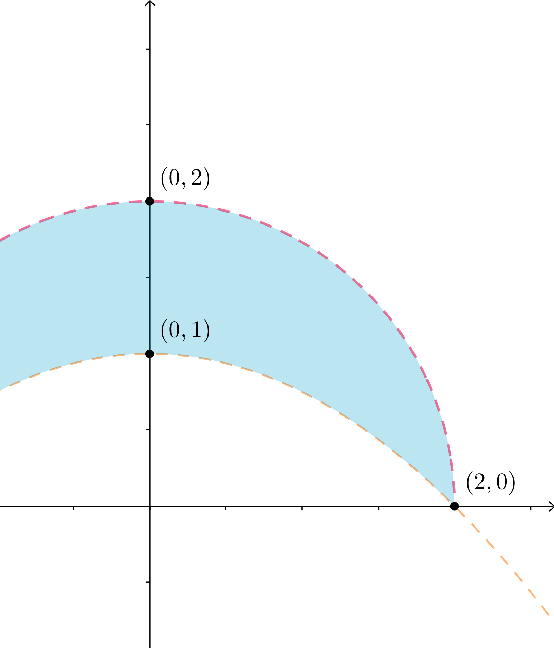
\includegraphics[width=7cm, height=9cm]{list23imgs/task 8.png}
    
    Изменим границы: $x \in [0, 2]$, на всём промежутке точки лежат между графиком окружности и параболы.
    
    
    Итого: $\displaystyle \int\limits_{0}^{2} dx \int\limits_{1 - x^2 / 4}^{\sqrt{4 - x^2}} f(x,y)dy$.
    
    \section*{Изменив порядок интегрирования, вычислите интеграл}
    
    \subsection*{Задача 9}
    
    $\int\limits_{0}^{1} dy \int\limits_{0}^{1 - y} e^{-x^2 + 2x + 1} dx.$
    
    Чтобы изменить порядок интегрирования, нужно знать, что представляет собой $D$.
    
    $y \in [0,1]$, и точки лежат под прямой $y = -x + 1$.
    
    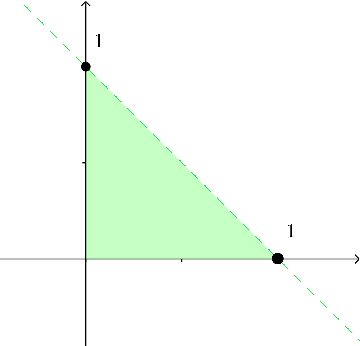
\includegraphics[width=4cm, height=5cm]{list23imgs/task 9.png}
    
    Изменяем порядок: $\int\limits_{0}^{1} dx \int\limits_{0}^{1 - x} e^{-x^2 + 2x + 1} dy = 
    \int\limits_{0}^{1} e^{-x^2 + 2x + 1}  \int\limits_{0}^{1 - x} dy \, dx =
    \int\limits_{0}^{1} e^{-(x - 1)^2 + 2} \; \, (1 - x) \, dx.$  
    
    Замена $\begin{cases}
    t = (x - 1)^2 = x^2 - 2x + 1;\\
    dt = (2x - 2)dx;\\
    dx = dt/(2x - 2);\\
    \text{границы становятся } (1, 0).
    \end{cases}$
    
    $\int\limits_{1}^{0} e^{-t + 2} \left( \frac{1 - x}{2x - 2}\right) dt = \int\limits_{1}^{0} e^{-t + 2} \left( - \frac{1}{2}\right) dt = -\frac{e^2}{2} \int\limits_{1}^{0} e^{-t} dt = -\frac{e^2}{2} \, \, \left(-e^{-t} \Bigg|_{t = 1}^{0} \right)=  \frac{-e^2(-e^0 + e^{-1})}{2} = \frac{e^2 - e}{2}.$
    
    \subsection*{Задача 10}
    \begin{flalign*}
        & \int \limits_0^2 x^2 dx \int \limits_x^2 \ln(1 + y^2) dy = \text{ пристально смотрим на рисунок } = 
        \int \limits_0^2 \int \limits_0^y x^2 \ln(1 + y^2) dx dy = \\
        & = \int \limits_0^2 \ln(1 + y^2) dy \int \limits_0^y x^2 dx =
        \int \limits_0^2 \ln(1 + y^2) dy \left( \left. \frac{x^3}{3} \right|_0^y \right) = 
        \frac{1}{3} \int \limits_0^2 \ln(1 + y^2) y^3 dy = \\
        & = \left\{ \begin{array} {ll}
            u = \ln(1 + y^2) & \Rightarrow u' = \frac{2y}{1 + y^2} \\
            v' = y^3 & \Rightarrow v = \frac{y^4}{4} 
        \end{array}  \right\} = 
        \frac{1}{3} \left. \ln(1 + y^2) \frac{y^4}{4} \right|^2_0 -
        \frac{1}{3} \int \limits_0^2 \frac{y^4}{4} \frac{2y}{1 + y^2} dy = 
        \left\{ \begin{array} {l}
            t = 1 + y^2 \\
            dt = 2y dy \\
            dy = \frac{dt}{2y} 
        \end{array}  \right\} = \\
        & = \frac{1}{3} \left( 4 \ln(5) - 0 \right) - \frac{1}{6} \int \limits_1^5 \frac{y^5}{t} \frac{dt}{2y} = 
        \frac{4}{3} \ln(5) - \frac{1}{12} \int \limits_1^5 \frac{(y^4 + 2y^2 + 1) - (2y^2 - 2) + 1}{t} dt = \\
        & = \frac{4}{3} \ln(5) - \frac{1}{12} \int \limits_1^5 \frac{t^2 - 2t + 1}{t} dt = 
        \frac{4}{3} \ln(5) - \frac{1}{12} \left( \int \limits_1^5 t dt - 2 \int \limits_1^5 dt + \int \limits_1^5 \frac{dt}{t}  \right) = \\
        & = \frac{4}{3} \ln (5) - \frac{1}{12} \left( \left( \frac{25}{2} - \frac{1}{2} \right) -
        2 (5 - 1) + \ln(|t|)\big|^5_1 \right) = \frac{4}{3} \ln(5) - \frac{1}{12} \left( 12 - 8 + \ln(5) \right) = \\
        & = \frac{4}{3} \ln(5) - \frac{1}{3} - \frac{\ln(5)}{12} = \pmb{\frac{5\ln(5)}{4} - \frac{1}{3}}
        % \frac{1}{3} \int \limits_0^2 \frac{y^4}{4} y^3 dy = \\
        % & = \frac{1}{3} \left( 4 \ln(5) - 0 \right) - \frac{1}{12} \left. \frac{y^8}{8} \right|^2_0 =
        % \frac{4}{3} \ln(5) - \frac{8}{3} 
    \end{flalign*}
    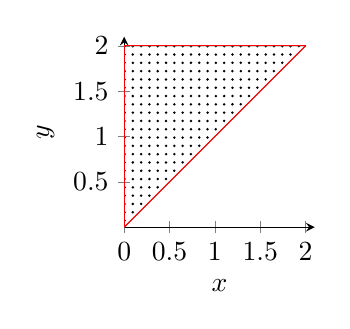
\begin{tikzpicture} 
        \begin{axis}[axis lines=center, xlabel={$x$}, ylabel={$y$},
                        xlabel near ticks, ylabel near ticks, hide obscured x ticks=false,
                        xmin=0, xmax=2.1, ymin=0, ymax=2.1,
                        width=4cm, height=4cm]
            \draw[color=red] (axis cs:0, 0) -- (axis cs:0, 2);
            \addplot [name path=A, domain=0:2, color=red] {2}; 
            \addplot [name path=B, domain=0:2, color=red, samples=50] {x}; 
            \addplot [pattern=dots, draw=gray] fill between[of=A and B];
        \end{axis} 
    \end{tikzpicture} 
    
    \subsection*{Задача 11}
    
    $\int\limits_{0}^{\pi} x dx \int\limits_{x}^{\pi} \frac{\sin y}{y} dy.$ Как всегда, ищем $D$ с помощью границ интегрирования.
    
    
    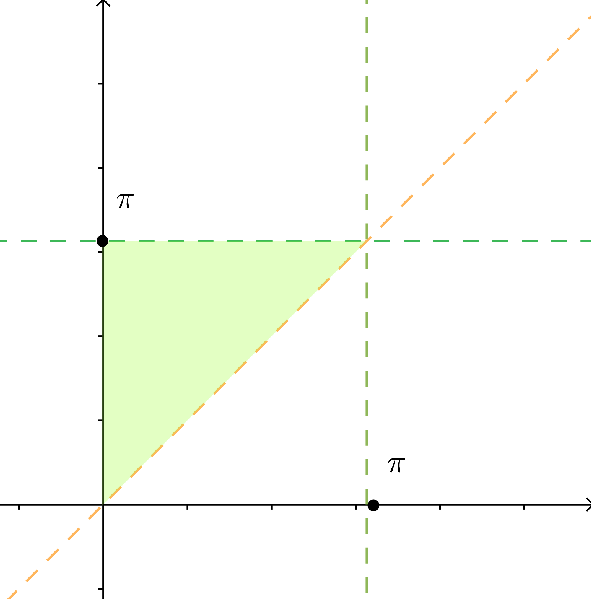
\includegraphics[width=6cm, height=6cm]{list23imgs/task_11.png}
    
    Тогда, изменив порядок, получим: $\int\limits_{0}^{\pi} dy \int\limits_{0}^{y} x \frac{\sin y}{y} dx = \int\limits_{0}^{\pi} \frac{\sin y}{y} dy \int\limits_{0}^{y} x  dx = \int\limits_{0}^{\pi} \frac{\sin y}{y}  \, \frac{y^2}{2} \, dy = \frac{1}{2} \int\limits_{0}^{\pi} (y \sin y) \, dy.$
    
    Интегрируем по частям.
    
        
    $\begin{cases}
    f = y \implies df = dy;\\
    g = -\cos y \implies dg = \sin y\, dy
    \end{cases}$
    
    $\frac{1}{2} \left(f \cdot g \Bigg|_{0}^{\pi} \right) - \frac{1}{2} \int\limits_{0}^{\pi} g \cdot df  =
    \frac{1}{2} \left(-y \cos y \Bigg|_{0}^{\pi} \right) - \frac{1}{2} \int\limits_{0}^{\pi} - \cos y dy = 
    \frac{1}{2} \left(-y \cos y \Bigg|_{0}^{\pi} \right) + \frac{1}{2}  \left(\sin y \Bigg|_{0}^{\pi} \right) = \frac{\pi}{2}.$
    
    % \subsection*{Задача 12}
    
    \section*{Вычислите интеграл}
    
    \subsection*{Задача 13}
    
    $\displaystyle\iint\limits_D x^3 y^5 dx dy, \; D = \{(x,y) \; : \; |x| + |y| \leq 1\}.$
    
    Наше множество $D$ -- это следующий квадрат:
    
    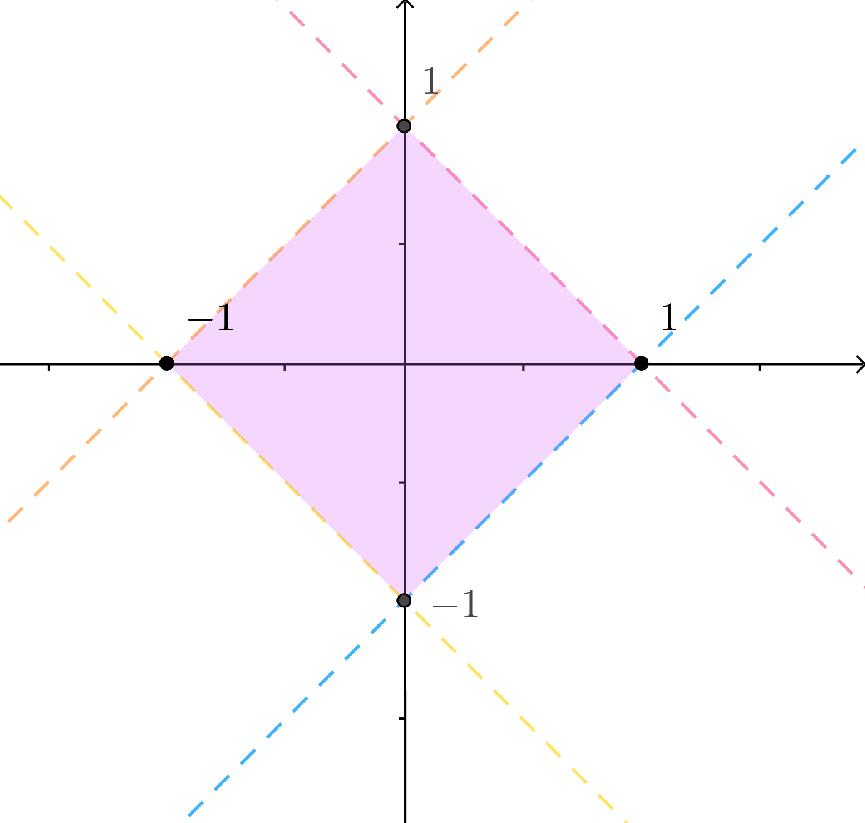
\includegraphics[width=6cm, height=6cm]{list23imgs/task 13.png}
    
    Зная $D$, можем увидеть границы интегрирования:
    
    
    $\displaystyle\int\limits_{-1}^{0} dx  \int\limits_{-1 -x}^{1 + x}x^3y^5 dy + \int\limits_{0}^{1} dx \int\limits_{-1 + x}^{1 - x} x^3y^5 dy = \int\limits_{-1}^{0} x^3 dx \int\limits_{-1 -x}^{1 + x} y^5 dy + \int\limits_{0}^{1} x^3 dx \int\limits_{-1 + x}^{1 - x} y^5 dy = \int\limits_{-1}^{0} x^3 \left( \frac{y^6}{6} \Bigg|_{y = -1 - x}^{1 + x} \right)dx +  \\
    \int\limits_{0}^{1} x^3 \left( \frac{y^6}{6} \Bigg|_{y = -1 + x}^{1 - x} \right)dx =
    \int\limits_{-1}^{0} x^3  \left( \frac{(1 + x)^6}{6} - \frac{(-1 - x)^6}{6}\right)dx + \int\limits_{0}^{1} x^3 \left(\frac{(1 - x)^6}{6} - \frac{(- 1 + x)^6}{6} \right) dx =0.
    $
    
    \subsection*{Задача 14}
    $D = \left\{ (x, y): x^2 + y^2 \leq 9 \right\} \;\;\;\;\;\; \iint \limits_D \sgn \left( x^2 + y^2 - 4 \right) dx dy$ 

    Заметим, что $D$ описывает множество точек круга с радиусом $3$, а подынтегральная функция принимает значение 
    $-1$ на точках круга радиусом $2$ и значение $1$ на всех остальных точках. 
    Получается задачу можно решать не через матан а через геому, чем мы и займемся.

    $\iint \limits_D \sgn \left( x^2 + y^2 - 4 \right) dx dy = - 1 (\pi 2^2) + 1 (\pi 3^2 - \pi 2^2) = \pi$

    % \subsection*{Задача 15}
    
    \subsection*{Задача 16}
    
    $\iint\limits_D xy \, dxdy$, $D$ ограничена осями координат и кривой $\begin{cases} 
    x = \cos^3 t;\\
    y = \sin^3 t
    \end{cases} t \in [0, \pi / 2].$
    
    Заметим, что при данных ограничениях $t$ однозначно выразим через $x \Rightarrow y$  тоже однозначно выразим через $x$.
    
    Тоесть $y = \varphi(x)$.
    
    На $[0, \pi/2]$ $x$ принимает значения от $0$ до $1$. Если $D$ ограничено осями координат и графиком $\varphi(x)$, то $y \in [0, \varphi(x)]$ при фиксированном $x$  (ибо $y$ неотрицателен при $t \in [0, \pi/2]$).
     
     Так что пределы интегрирования знаем:
     
     $\int\limits_{0}^{1} dx \int\limits_{0}^{\varphi(x)} xy \; dy = \int\limits_{0}^{1} dx \left( \frac{xy^2}{2}  \Bigg|_{0}^{\varphi(x)}
     \right)  = \int\limits_{0}^{1}  \left( \frac{x \cdot \varphi^2(x)}{2}\right) dx.$
     
     Пришло время подставить параметр: $\begin{cases} x = \cos^3 t;\\
     \varphi(x) = \sin^3 t;\\
     dx = 3 \cos^2 t \cdot (-\sin t) \, dt;\\
     \text{пределы интегрирования теперь } [\pi/2, 0]
     \end{cases}$
     
     $\int\limits_{\pi/2}^{0} -\frac{3}{2} \cos^3 t \cdot \sin^6 t \cdot \cos^2 t \cdot \sin t \, dt = \frac{3}{2} \int\limits_{0}^{\pi/ 2} \cos^5 t\cdot \sin^7 t \, dt.$
     
     Идея: отщепим один множитель (синус или косинус), загоним его под дифференциал. И введем новую переменную:
     
     $\begin{cases}
     \cos t \,dt = d \sin t;\\
     u := \sin t;\\
     \cos ^ 4 t = (1 - u^2)^2;\\
     \text{пределы интегрирования теперь } [0, 1]
     \end{cases}$
    
    $\frac{3}{2} \int\limits_{0}^{1} (1 - u^2)^2 \cdot u^7 \, du = \frac{3}{2} \int\limits_{0}^{1} u^7 - 2 u^9 + u^{11} \, du = \frac{3}{2} \left( \frac{u^8}{8} - \frac{u^{10}}{5} + \frac{u^{12}}{12} \Bigg|_{u = 0}^{1}\right) = \frac{3}{2} \left(\frac{1}{8} - \frac{1}{5} + \frac{1}{12}\right) = \frac{3}{2} \cdot \frac{15 - 24 + 10}{120} = \frac{1}{80}.$
    
    \textit{P.s. тут картинка не нужна!}
    
    
    \section*{Предполагая функцию $f$ непрерывной на $D$, измените порядок интегрирования в повторном интеграле
    всеми возможными способами}
    
    \subsection*{Задача 17}
    
    $\int\limits_{0}^{1} dx \int\limits_{0}^{1 - x} dy \int\limits_{0}^{1 - x - y} f(x, y, z) dz.$
    
    Если есть 3 переменных, то порядок интегрирования может быть задан $3! = 6$ возможными способами. Нужно найти оставшиеся 5.
    
    Как и в 2-мерном случае, попытаемся восстановить множество $D$.
    
    $x \in [0,1]$ -- внешний интеграл.
    
    В плоскости $Oxy$ образуется треугольник между осями координат и прямой $y = -x + 1.$ 
    
    Так как $z \leq 1 - x - y,$ то нас будет интересовать участок под плоскостью $z + x + y = 1.$ Итого получаем пирамидку:
    
    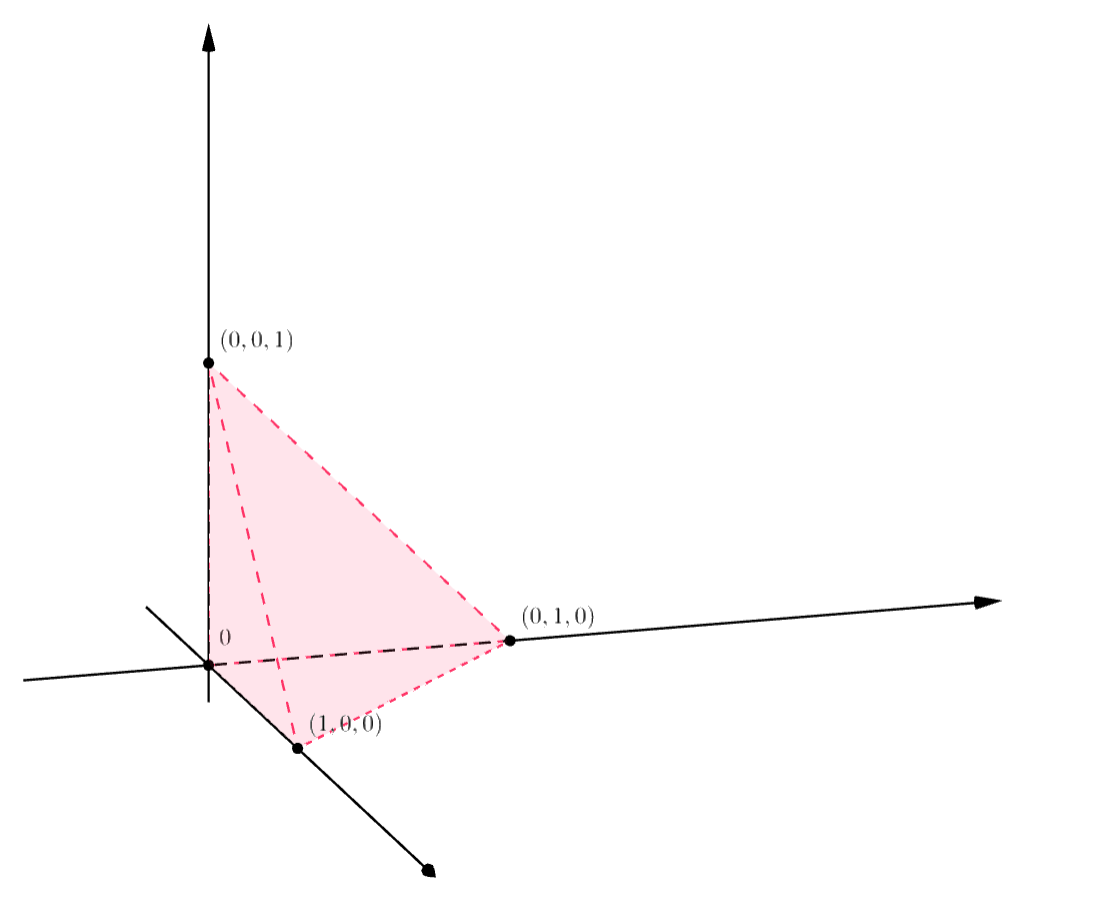
\includegraphics[width=14cm, height=12cm]{list23imgs/task 17.png}
    
    Теперь всё стало очень просто, потому что наша пирамидка симметрична относительно любой замены координат (друг на друга). Значит, можем просто изменить координаты в формуле побуквенно. Погнали:
    
        
    $\int\limits_{0}^{1} dx \int\limits_{0}^{1 - x} dz \int\limits_{0}^{1 - x - z} f(x, y, z) dy.$
    
        
    $\int\limits_{0}^{1} dy \int\limits_{0}^{1 - y} dx \int\limits_{0}^{1 - x - y} f(x, y, z) dz.$
    
    $\int\limits_{0}^{1} dy \int\limits_{0}^{1 - y} dz \int\limits_{0}^{1 - z - y} f(x, y, z) dx.$
        
    $\int\limits_{0}^{1} dz \int\limits_{0}^{1 - z} dx \int\limits_{0}^{1 - x - z} f(x, y, z) dy.$
    
    $\int\limits_{0}^{1} dz \int\limits_{0}^{1 - z} dy \int\limits_{0}^{1 - z - y} f(x, y, z) dx.$
    
    \subsection*{Задача 18}
    \begin{flalign*}
        & \int_0^1 dx \int_0^x dy \int_0^y f(x, y, z) dz \;\;\;\;\;\; \text{Порядок интегрирования (x, y, z)} \\
        & \text{Видим, что} \begin{cases} 
            x, y, z \in [0, 1] \\
            y \leq x; \;\; z \leq y \;\; z \leq x
        \end{cases} \text{ — это помогает шафлить порядок интегрирования} \\
        & \text{Пристально смотрим на картинку, начинаем менять порядок: } \\
        & \mathbf{(x, z, y) \colon} \int_0^1 dx \int_0^x dz \int_z^x f(x, y, z) dy \\
        & \mathbf{(y, x, z) \colon} \int_0^1 dy \int_y^1 dx \int_0^y f(x, y, z) dz \\
        & \mathbf{(y, z, x) \colon} \int_0^1 dy \int_0^y dz \int_y^1 f(x, y, z) dx \\ 
        & \mathbf{(z, x, y) \colon} \int_0^1 dz \int_z^1 dx \int_z^x f(x, y, z) dy \\ 
        & \mathbf{(z, y, x) \colon} \int_0^1 dz \int_z^1 dy \int_y^1 f(x, y, z) dx \\ 
    \end{flalign*}
    Алгоритм действий для меня был выписать все известные отношения с уже введенными переменными и использовать самые строгие.
    Может быть в более потных примерах придется дробить интегралы на несколько, но лично я такое решать не хочу.

    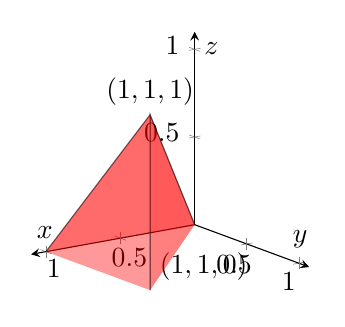
\begin{tikzpicture} 
        \begin{axis} [width=6cm, xlabel={$x$}, ylabel={$y$}, zlabel={$z$}, axis lines=center, axis equal image,
                        view={145}{15},
                        xmin=0, xmax=1.1, ymin=0, ymax=1.1, zmin=0, zmax=1.1]
            \coordinate (O) at (axis cs:0, 0, 0);
            \coordinate[label={$(1, 1, 1)$}] (A) at (axis cs:1, 1, 1);
            \coordinate (B) at (axis cs:1, 0, 0);
            \coordinate[label=above right:{$(1, 1, 0)$}] (C) at (axis cs:1, 1, 0); 
            
            \draw[fill=red, opacity=0.5] (O) -- (A) -- (C); 
            \draw[fill=red, opacity=0.3] (O) -- (A) -- (B); 
            \draw[fill=red, opacity=0.4] (C) -- (A) -- (B); 
        \end{axis} 
    \end{tikzpicture} 
    
    % \subsection*{Задача 19}
    
    % \subsection*{Задача 20}
    
    \subsection*{Задача 21}
    
    $\displaystyle \int\limits_{-1}^{1} dx \int\limits_{-\sqrt{1 - x^2}}^{\sqrt{1 - x^2}} dy \int\limits_{0}^{1 - \sqrt{1 - x^2 - y^2}} f(x,y,z) dz.$
    
    Ищем $D$. 
    
    $x \in [-1, 1]$, в плоскости $Oxy$ образуется круг радиусом 1.
    
    Что говорят пределы интегрирования по $z$? Во-первых, $z \geq 0$. Во вторых -- нас интересует часть пространства под поверхностью $(z-1)^2 + y^2 + x^2 = 1.$ Это -- сфера с центром в $(0, \, 0, \,1)$ и радиусом 1.
    
    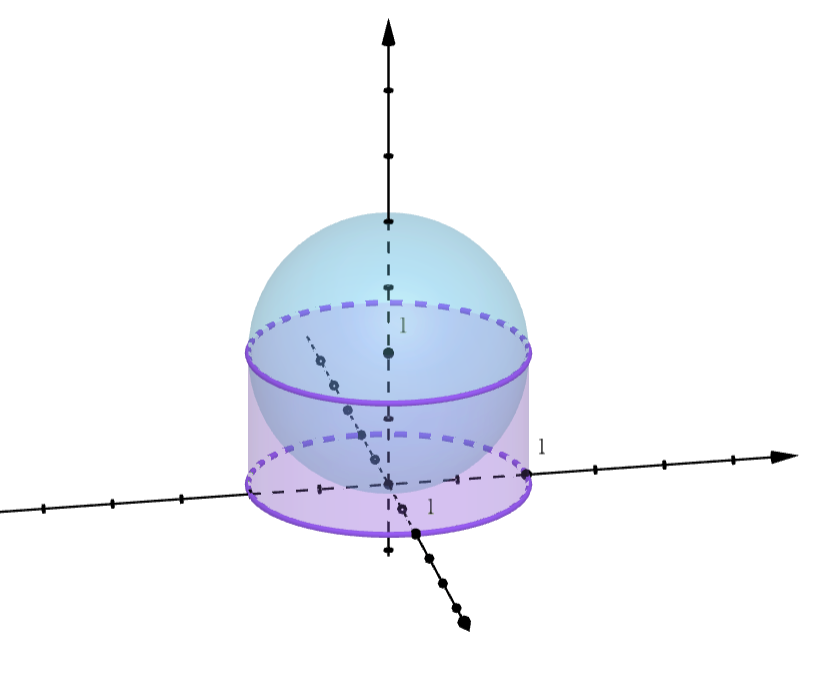
\includegraphics[width=14cm, height=12cm]{list23imgs/task 21.png}
    
    \textit{Нам нужны точки внутри этого цилиндра, но вне полушара.}
    
    Множество симметрично относительно замены $x$ на $y$, но несимметрично относительно других замен.
    
    Попробуем интегрировать в порядке $zxy$. $z \in [0, 1].$  При фиксированном $z_0$ получается такое сечение $D$:
    
    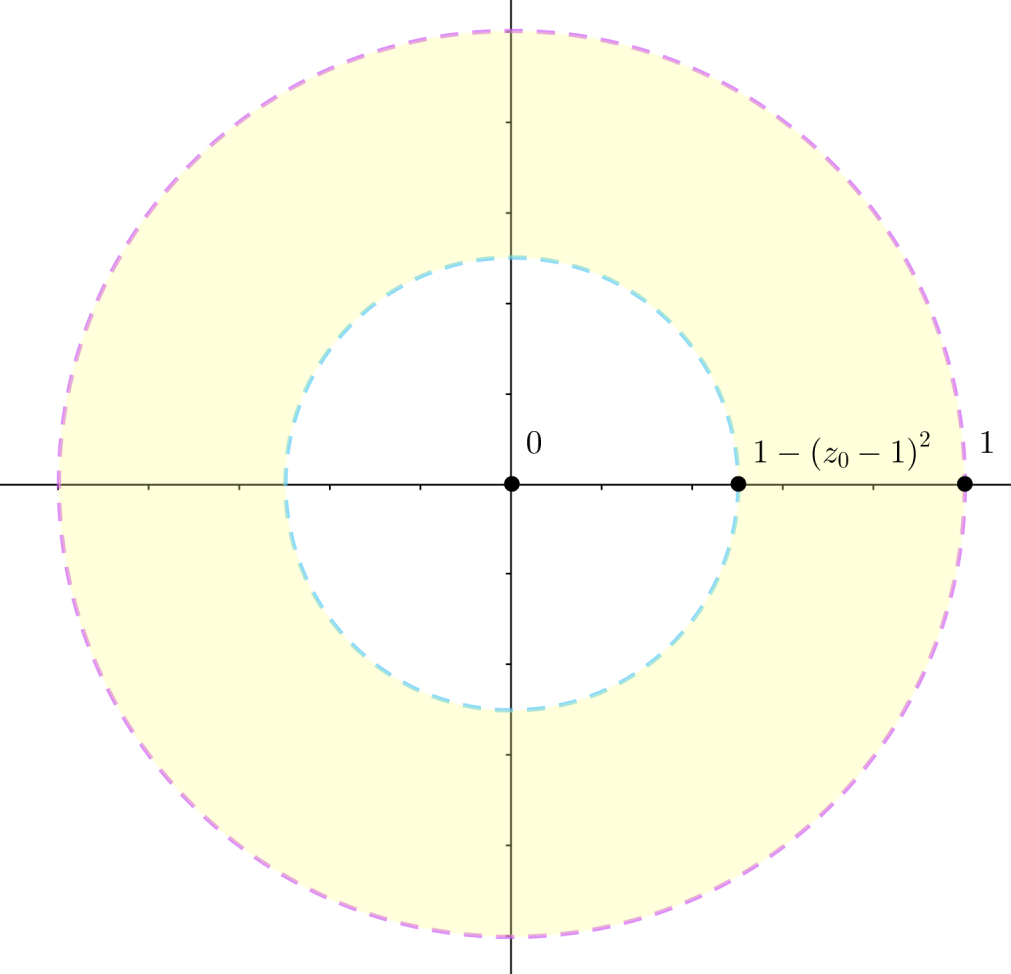
\includegraphics[width=8cm, height=8cm]{list23imgs/task 21-2.png}
    
    Радиус внутренней окружности = $1 - (z_0 - 1)^2,$ чтобы выполнилось неравенство  $(z - 1)^2 + x^2 + y^2 \geq 1.$ 
    
    Интегрирование по $x$ приводит к рассмотрению 3 однородных участков (до перекрытия внутренней окружностью, в перекрытии, и после перекрытия).
    
    Итого: $\int\limits_{0}^{1} dz \left(
    \int\limits_{-1}^{-\sqrt{1 - (z - 1)^2}} dx \int\limits_{-\sqrt{1 - x^2}}^{\sqrt{1 - x^2}} f \, dy +
    2 \cdot \int\limits_{-\sqrt{1 - (z - 1)^2}}^{\sqrt{1 - (z - 1)^2}} dx \;  \int\limits_{\sqrt{(1 - z^2) - x^2}}^{\sqrt{1 - x^2}} f \, dy + 
    \int\limits_{\sqrt{1 - (z - 1)^2}}^{1}dx \int\limits_{-\sqrt{1 - x^2}}^{\sqrt{1 - x^2}} f \, dy
    \right)$
    
    Все остальные случаи можно получить, использую симметрию множества по $x$ и $y$.
    
    \subsection*{Задача 22}
    \begin{flalign*}
        & \int\limits_0^1 dx \int\limits_{-\sqrt{1 - x^2}}^{\sqrt{1 - x^2}} dy 
        \int\limits_{-\sqrt{1 - x^2 - y^2}}^{\sqrt{1 - x^2 - y^2}} f(x, y, z) dz \\
        & x \in [0, 1]; \;\; -\sqrt{1 - x^2} \leq y \leq \sqrt{1 - x^2} \;\; \implies \;\; y^2 \leq 1 - x^2 \;\;
        \implies \;\; x^2 + y^2 \leq 1 \\
        & -\sqrt{1 - x^2 - y^2} \leq z \leq \sqrt{1 - x^2 - y^2} \;\; \implies \;\; 
        z^2 \leq 1 - x^2 - y^2 \;\; \implies \;\; x^2 + y^2 + z^2 \leq 1 \\
        & \text{Получается это единичная полусфера с центром в нуле, что все иксы неотрицательные.} \\
        & \mathbf{(x, z, y) \colon} 
        \int\limits_0^1 dx \int\limits_{-\sqrt{1 - x^2}}^{\sqrt{1 - x^2}} dz 
        \int\limits_{-\sqrt{1 - x^2 - z^2}}^{\sqrt{1 - x^2 - z^2}} f(x, y, z) dy \\
        & \mathbf{(y, x, z) \colon} 
        \int\limits_{-1}^1 dy \int\limits_0^{\sqrt{1 - y^2}} dx 
        \int\limits_{-\sqrt{1 - x^2 - y^2}}^{\sqrt{1 - x^2 - y^2}} f(x, y, z) dz \\
        & \mathbf{(y, z, x) \colon} 
        \int\limits_{-1}^1 dy \int\limits_{-\sqrt{1 -y^2}}^{\sqrt{1 - y^2}} dz 
        \int\limits_{0}^{\sqrt{1 - y^2 - z^2}} f(x, y, z) dx \\
        & \mathbf{(z, x, y) \colon}
        \int\limits_{-1}^1 dz \int\limits_{0}^{\sqrt{1-z^2}} dx 
        \int\limits_{-\sqrt{1 - x^2 - z^2}}^{\sqrt{1 - x^2 - z^2}} f(x, y, z) dy \\
        & \mathbf{(z, y, x) \colon} 
        \int\limits_{-1}^1 dz \int\limits_{-\sqrt{1-z^2}}^{\sqrt{1-z^2}} dy \int\limits_0^{\sqrt{1-y^2-z^2}} f(x, y, z) dx
    \end{flalign*}
    Рисовать сферу мне лень, но тут, впрочем, рисунок ни на что и не влиял
\end{document}
